\DocumentMetadata{
  lang        = en-US,
  pdfversion  = 2.0,
  pdfstandard = ua-2,
  tagging     = on,
  tagging-setup = {math/setup=mathml-SE}
}
\documentclass[12pt]{article}
\usepackage{amsmath, amssymb, amsthm, xcolor, graphicx, colortbl}
\usepackage{siunitx}

% SciencePlots defaults for matplotlib-style exports
\usepackage{caption}
\captionsetup{labelformat=empty}

\usepackage{geometry}
\geometry{
	letterpaper,
	total={6.5in, 9in},
	left=1in,
	top=1in,
}

\usepackage{fontspec}
\setmainfont{Libertinus Serif}
\setsansfont{Libertinus Sans}
\setmonofont{Libertinus Mono} 

\usepackage{hyperref}

\parskip = 0.125in
\parindent = 0.0in

\everymath{\displaystyle}

% Integral Evaluated at | operator, \Eval{anti-derivative}{a}{b}
\newcommand*\Eval[3]{\left.#1\right\rvert_{#2}^{#3}}

% Equals with LH above it for L'Hopital's Rule
\newcommand\eqLH{\mathrel{\stackrel{\makebox[0pt]{\mbox{\normalfont\tiny LH}}}{=}}}
\newcommand{\eqwith}[1]{\mathrel{\overset{\scriptstyle\text{#1}}{=}}}

% Force limits-style subscripts on \lim.
\renewcommand{\lim}{\mathop{\mathrm{lim}}\limits}

\newcommand{\RR}{\mathbb{R}}
\newcommand{\NN}{\mathbb{N}}
\newcommand{\ZZ}{\mathbb{Z}}
\newcommand{\QQ}{\mathbb{Q}}
\newcommand{\CC}{\mathbb{C}}

% Based on Paul Tol's Vibrant color scheme 
% https://sronpersonalpages.nl/~pault/
\definecolor{VibrantBlue}{HTML}{0077bb}
\definecolor{VibrantCyan}{HTML}{33bbee}
\definecolor{VibrantTeal}{HTML}{009988}
\definecolor{VibrantOrange}{HTML}{ED6F26}
\definecolor{VibrantRed}{HTML}{cc3311}
\definecolor{VibrantMagenta}{HTML}{ee3377}
\definecolor{VibrantGray}{HTML}{757575}
\definecolor{TextBlue}{HTML}{0077bb}
\definecolor{TextTeal}{HTML}{008575}
\definecolor{TextOrange}{HTML}{C85014}
\definecolor{TextMagenta}{HTML}{E71361}
\definecolor{GradRed}{HTML}{DC050C}

% Pre-notes intentionally leave certain content blank, to be filled in on the post-notes.
% For screen readers, we mark these blank spaces as artifacts so that they are not read aloud in the pre-notes.
\newcommand{\mathvidartifact}[1]{%
  \ifdefined\tagpdfmc
    \tagpdfmc{artifact}#1\tagpdfmcend
  \else
    #1%
  \fi
}

% Styled macros for Definitions, Theorems, and Corollaries.
\newcommand{\msColor}[2]{\textcolor{#1}{#2}}
\newcommand{\msDef}[1]{\textbf{\msColor{TextBlue}{Definition}}\if\relax\detokenize{#1}\relax\textbf{\msColor{black}{:}}\else\textbf{\;\msColor{black}{#1:}}\fi}
\newcommand{\msThm}[1]{\textbf{\msColor{TextTeal}{Theorem}}\if\relax\detokenize{#1}\relax\textbf{\msColor{black}{:}}\else\textbf{\;\msColor{black}{#1:}}\fi}
\newcommand{\msThmNamed}[1]{\if\relax\detokenize{#1}\relax\textbf{\msColor{TextTeal}{:}}\else\textbf{\msColor{TextTeal}{#1:}}\fi}
\newcommand{\msCor}[1]{\textbf{\msColor{TextTeal}{Corollary}}\if\relax\detokenize{#1}\relax\textbf{\msColor{black}{:}}\else\textbf{\;\msColor{black}{#1:}}\fi}
\newcommand{\msProof}{\textbf{\msColor{TextTeal}{Proof: }}}
\newcommand{\msAlgorithm}[1]{\textbf{\msColor{TextOrange}{#1: }}}
\newcommand{\msReadAs}{\textbf{\msColor{TextMagenta}{Read Aloud As: }}}
\newcommand{\msRead}{\textbf{\msColor{TextMagenta}{Read Aloud: }}}
\newcommand{\msCareful}{\textbf{\msColor{GradRed}{Careful: }}}

\AddToDocumentProperties[hyperref]{pdftitle}{Evaluating Definite Integrals using Graphs and Geometry Pre-notes}
\AddToDocumentProperties[hyperref]{pdfauthor}{Sean Groathouse}
\AddToDocumentProperties[hyperref]{pdfsubject}{Calculus I}
\AddToDocumentProperties[hyperref]{pdfkeywords}{definite integral, area under a curve, net area}
\newcommand{\prenotephantom}[1]{\mathvidartifact{\begingroup\color{white}#1\endgroup}}

\begin{document}
\begingroup\fontsize{16.0}{19.2}\selectfont
\begin{center}
\textbf{Evaluating Definite Integrals using Graphs and Geometry}
\end{center}
\endgroup

In this lesson, we will use graphs and geometry to evaluate definite integrals.

Say we want to evaluate $\int_a^b c \,dx$, where $c$ is a constant. The definite integral gives the net area bounded by the graph of $y=c$ and the $x$-axis.

\vspace{-0.5cm}

\begin{center}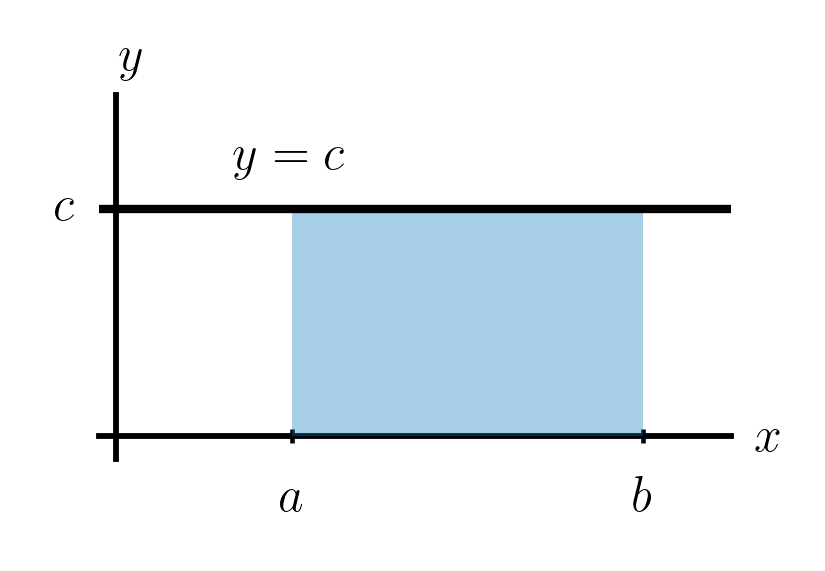
\includegraphics[width=2.75in,alt={Graph of y equals c, a horizontal line at height c. The region from x equals a to x equals b is shaded as a rectangle with width b minus a and height c.}]{assets/plot_pre_0.png}\end{center}

\vspace{-0.5cm}

\prenotephantom{The net area is a rectangle with width \prenotephantom{$b-a$} and height \prenotephantom{$c$}. The area is \prenotephantom{$c(b-a)$}. So,
\[\boxed{\prenotephantom{\int_a^b c\,dx = c(b-a)}}\]}

\textbf{Example 1: } Use geometry to evaluate $\int_1^5 (x+2)\,dx$.

\vspace{-0.5cm}

\begin{center}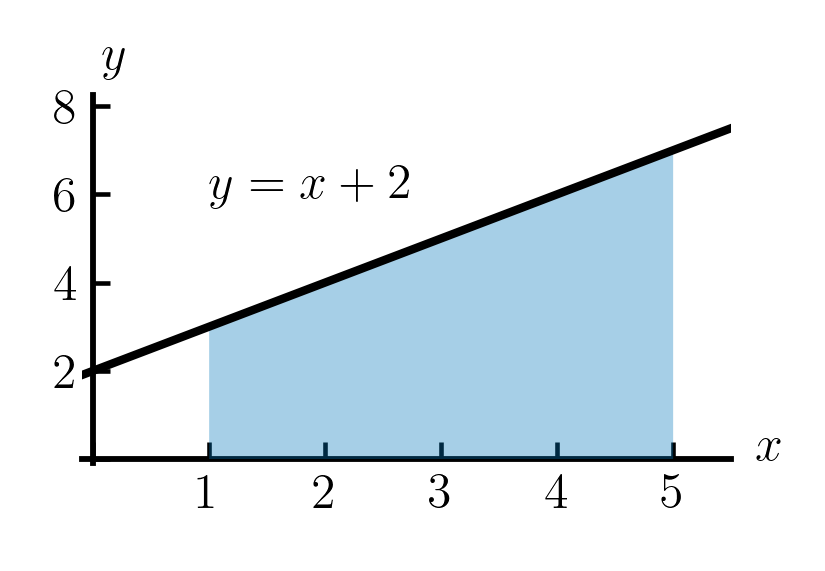
\includegraphics[width=2.75in,alt={Graph of y equals x plus 2 on the interval from 1 to 5. The region under the curve is shaded as a trapezoid with vertical sides at x equals 1 and x equals 5.}]{assets/plot_pre_1.png}\end{center}

\vspace{-0.5cm}

\prenotephantom{\textbf{Solution: } The region under $y = x+2$ on $[1,5]$ is a trapezoid. The area of a trapezoid is $\dfrac{1}{2}(b_1+b_2)h$. This trapezoid is sideways, so the height runs along the $x$-axis: $h = 5-1=4$.
The bases are the vertical lengths $1+2=3$ and $5+2=7$. So,}

\begin{align*}
\phantom{\int_1^5 (x+2)\,dx = \frac{1}{2} (3+7)(4) = \boxed{20}}
\end{align*}

\newpage

\textbf{Example 2: } Use geometry to evaluate $\int_{-1}^4 (x-1)\,dx$.

\vspace{-0.5cm}

\begin{center}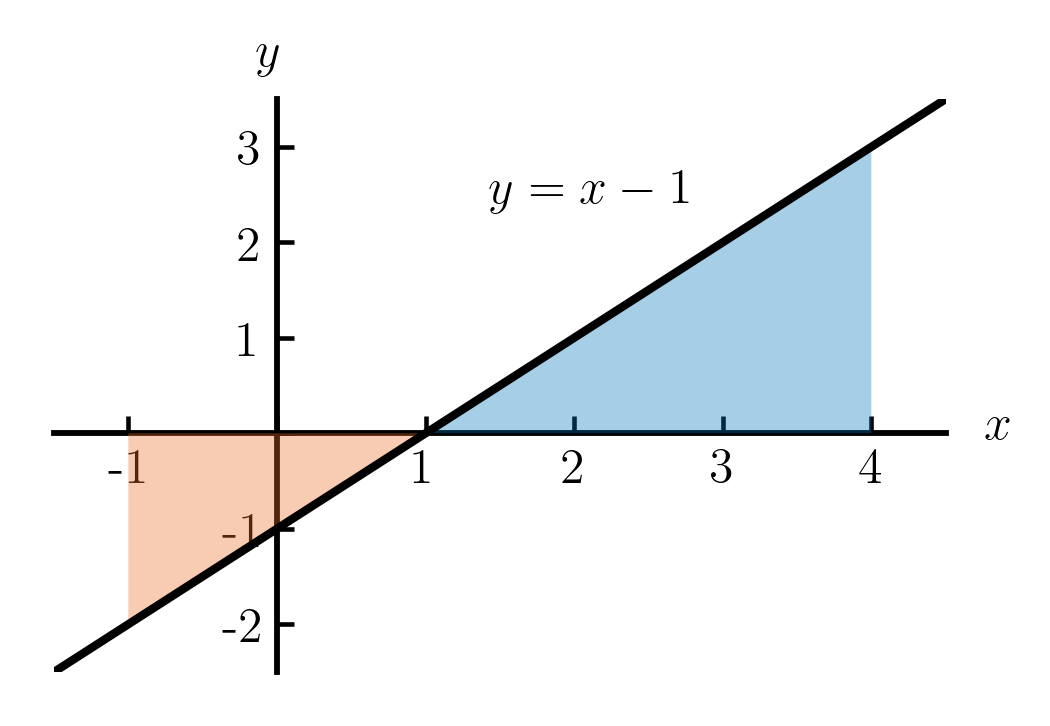
\includegraphics[width=3.5in,alt={Graph of the line y equals x minus 1 on the interval from negative 1 to 4. The line intersects the x-axis at x equals 1. From x equals 1 to 4, the line is above the x-axis, and the area below the line is a triangle shaded blue. From x equals negative 1 to 1, the line is below the x-axis, and the area between the line and the x-axis is a triangle shaded orange.}]{assets/plot_pre_2.png}\end{center}

\vspace{-0.5cm}

\prenotephantom{\textbf{Solution: } The definite integral gives the net area: the area of the triangle above the $x$-axis minus the area of the triangle below the $x$-axis. \\[0.25cm]
The triangle above the $x$-axis has base $4-1=3$ and height $3$, so the area is $\dfrac{1}{2}(3)(3)=\dfrac{9}{2}$. \\[0.25cm]
The triangle below the $x$-axis has base $1-(-1)=2$ and height $2$, so the area is $\dfrac{1}{2}(2)(2)=2$. \\[0.25cm]
The net area is $\dfrac{9}{2}-2=\dfrac{5}{2}$. So,}

\begin{align*}
\phantom{\int_{-1}^4 (x-1)\,dx = \boxed{\frac{5}{2}}}
\end{align*}

\vfill

\newpage

Now try these interactive problems on the website, to practice some new cases: an area under a curved function and using a graph with labeled areas to find a definite integral.

\textbf{Interactive Problem 1: } Use geometry to evaluate $\int_{-3}^3 \sqrt{9 - x^2}\,dx$.

\vspace{-0.5cm}

\begin{center}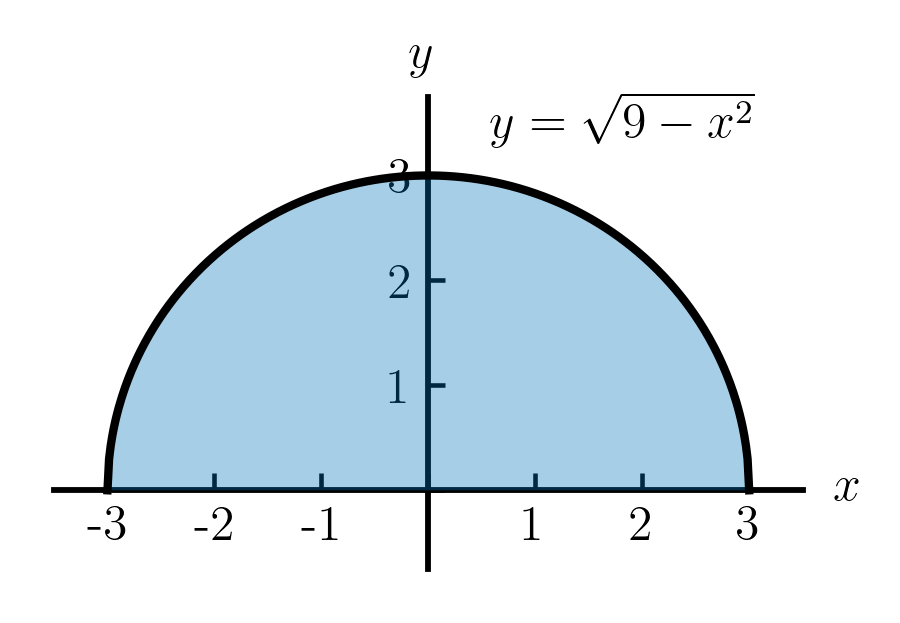
\includegraphics[width=3in,alt={Graph of y equals the square root of 9 minus x squared on the interval from negative 3 to 3. The region under the upper semicircle is shaded. The curve is the top half of a circle centered at the origin with radius 3.}]{assets/plot_pre_3.png}\end{center}

\vspace{-0.5cm}

\begin{enumerate}[item-label={(\alph*)}]
    \item On the graph, the definite integral $\int_{-3}^3 \sqrt{9-x^2}\,dx$ is the \prenotephantom{area of the semicircle.} \\[0.5cm]
    \item The formula for the area of a semicircle is \prenotephantom{$\frac{1}{2} \pi r^2$.} \\[0.5cm]
    \item The radius of the semicircle is \prenotephantom{$3$.} \\[0.5cm]
    \item Putting this all together, the definite integral is $\int_{-3}^3 \sqrt{9-x^2}\,dx = \prenotephantom{\frac{1}{2} \pi (3)^2 = \frac{9}{2} \pi.}$
\end{enumerate}

\vfill

\newpage

\textbf{Interactive Problem 2: } The graph shows the areas $A_1=3$, $A_2=5$, and $A_3=6$ of regions bounded by the graph of $y = f(x)$ and the $x$-axis. We will use the graph to find $\int_0^b f(x) \,dx$ and $\int_a^c f(x) \,dx$.

\begin{center}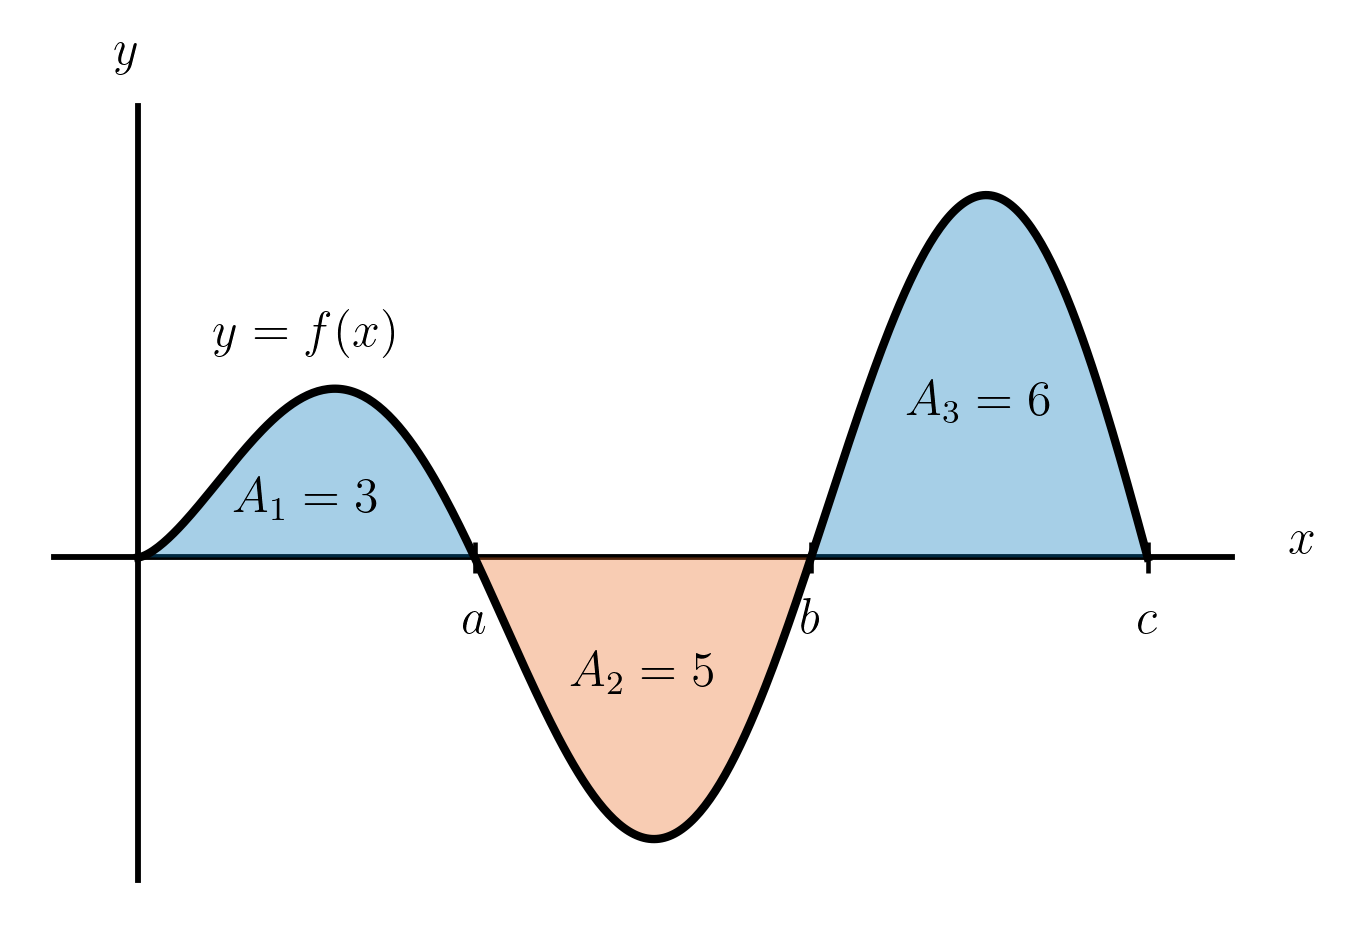
\includegraphics[width=4.5in,alt={Graph of a curved function y equals f of x from x equals 0 to points a, b, and c along the x-axis. The region from 0 to a is shaded above the x-axis and labeled A sub 1 equals 3. The region from a to b is shaded below the x-axis and labeled A sub 2 equals 5. The region from b to c is shaded above the x-axis and labeled A sub 3 equals 6.}]{assets/plot_pre_4.png}\end{center}

\begin{enumerate}[item-label={(\alph*)}]
    \item The areas involved in finding $\int_0^b f(x) \,dx$ are \prenotephantom{$A_1$ and $A_2$.} \\[0.5cm]
    \item $A_1$ counts as \prenotephantom{positive area.} \\[0.5cm]
    \item $A_2$ counts as \prenotephantom{negative area.} \\[0.5cm]
    \item So, $\int_0^b f(x) \,dx = \prenotephantom{A_1 - A_2 = 3 - 5 = -2.}$ \\[0.5cm]
    \item The areas involved in finding $\int_a^c f(x) \,dx$ are \prenotephantom{$A_2$ and $A_3$.} \\[0.5cm]
    \item The net area is $\int_a^c f(x) \,dx = \prenotephantom{-A_2 + A_3 = -5 + 6 = 1.}$
\end{enumerate}


\end{document}
